\chapter{Implementierung}
\printmyminitoc{1}

In diesem Kapitel wird die Implementierung des Rogue Devices beschrieben. Dabei wird auf die Verbindung des Rogue Devices
mit dem Controller und dem Schiff eingegangen. Zudem wird die Umsetzung der Kommunikation zwischen den einzelnen Komponenten
beschrieben. Dabei hat die Übersetzung von CAN-Bus Nachrichten eine wichtige Rolle gespielt.

\section{Umsetzung des Rogue Device}
Wie bereits in Kapitel \ref{sec:raspberrypi} beschrieben, wird ein Raspberry Pi 5 als Rogue Device benutzt. 
Als Betriebssystem wird Raspberry Pi OS benutzt. Der Standard Package Manager ist APT. Unter dessen Benutzung werden 
Python 3.12 und die benötigten Bibliotheken installiert. Damit sind die Vorraussetzungen für die weitere Implementierung
gesetzt.

\section{Verbindung Rogue Device - Controller} 

Im ersten Schritt wird der Spiele-Controller mit dem Raspberry Pi verbunden. Der Raspberry Pi wird mit Raspberry Pi OS betrieben.
Als Standard-Bluetooth-Treiber wird BlueZ\footnote{\href{https://www.bluez.org/}{BlueZ} (besucht am 02.01.2025)} verwendet. 
Dieser ist bereits vorinstalliert und muss 
nicht manuell installiert werden. Da es sich in diesem Fall um einen Xbox-Controllers handelt, wurde der Treiber
xboxdrv\footnote{\href{https://github.com/xboxdrv/xboxdrv}{xboxdrv} (besucht am 02.01.2025)} installiert. 
Diese können im APT-Repository gefunden werden.
Zusätzlich muss der Enhanced Re-Transmission Mode (ERTM) deaktiviert 
werden.\footnote{\href{https://wiki.debian.org/Gamepad\#Xbox\_Controllers\_over\_Bluetooth}{Debian Wiki} (besucht am 22.03.2025)} 
Dieser Modus ist standardmäßig aktiviert und
verhindert die korrekte Verbindung des Controllers, aufgrund eines Kompatibilitätsproblem.
Zusätzlich muss sichergestellt werden, dass die Firmware des Spiele-Controllers
auf dem aktuellen Stand ist. Um den Xbox-Controller zu verbinden, kann die graphische Benutzeroberfläche benutzt werden.
\\
Als Programmiersprache wird Python 3 benutzt. Die Sprache wurde gewählt, da für alle benötigten Funktionen bereits eine Bibliothek
existiert.
Die Struktur des Rogue Devices soll wie folgt aussehen:
\begin{figure}[H]
    \centering
    \includegraphics[scale=0.4]{images/piKonzept.png}
    \caption{Programmstruktur auf dem Rogue Device}
    \label{fig:structureRogueDevice}
\end{figure}

Für das im Rahmen der Arbeit entwickelte Programm \texttt{controllerInput.py} wird die Bibliothek \texttt{pygame} benutzt.
Eine Einordnung des entwickelten Programms in die Programmstruktur ist in Abbildung \ref{fig:structureRogueDevice} zu sehen.
Die Bibliothek ermöglicht es, Eingaben von einem Controller zu empfangen. Diese Eingaben
werden in Variablen gespeichert. Dabei gilt es zu beachten, dass der Gashebel oder die Ruderposition nicht
zu schnell verändert werden. Dies könnte zu einem unkontrollierten Verhalten des Schiffes oder zu Schäden führen. 
Daher werden diese Werte mit Tasten des
Controllers eingegeben, welche nicht nur eine binäre Eingabe haben. Diese werden als Achsen bezeichnet. Diese ermöglichen
eine stufenlose Eingabe. Bei einer vollständigen Eingabe soll die Gashebelposition nach 20 Sekunden 100\% erreichen.
So ist sichergestellt, dass die Gashebelposition nicht zu schnell verändert wird. Die Ruderposition soll nach 2 Sekunden
in jede Richtung jeweils 100\% erreichen. Dies ist ein Kompromiss zwischen Geschwindigkeit und Genauigkeit.

\section{Übersetzung Signale Controller - Schiff} \label{sec:signalControllerSchiff}

Wie in Abbildung \ref{fig:structureRogueDevice} zu sehen ist, erhält \texttt{controllerInput.py} die Signale des Xbox-Controllers 
erhält Variablen in Python interpretiert.
Diese Variablen müssen
dann in Nachrichten für den CAN-Bus umgewandelt werden. Hierfür wurde ein weiteres Programm entwickelt, welches die Übersetzung die 
Kodierung der CAN-Bus Nachrichten realisiert. Dieses Programm wird \texttt{canInterpreter.py} genannt.
Damit die beiden Programme miteinander kommunizieren
können, wird Inter-Process-Communication (IPC) benutzt. Als Methode werden hierbei Pipes benutzt. Diese sind einfach zu implementieren und haben
eine automatische Synchronisierung zwischen den Prozessen. Dadurch müssen Prozesse nicht aufeinander warten und können weiterarbeiten. 
Die Synchronisierung wird durch den Puffer der Pipe sichergestellt \cite{Venkataraman2015}. 
Wenn dieser voll ist, wird der schreibende Prozess angehalten, bis der
lesende Prozess den Puffer geleert hat. Dies ist ein einfaches und effizientes Verfahren, 
um die beiden Prozesse zu synchronisieren. Im Rahmen dieser Arbeit dafür ein weiteres Programm entwickelt, welches die Kommunikation
zwischen \texttt{controllerInput.py} und \texttt{canInterpreter.py} ermöglicht. Dieses Programm wird \texttt{mainProcess.py} genannt und 
benutzt die Bibliothek \texttt{subprocess}. Dabei werden die beiden Prozesse als Subprozesse gestartet. Die Ausgaben von 
\texttt{controllerInput.py} werden in die Pipe geschrieben und von \texttt{canInterpreter.py} als Eingaben gelesen.

\subsection{Eingabe-Interface}
Durch die begrenzte Zeit dieser Arbeit, wurde die Rückmeldung mit Vibrationen im Xbox-Controller implementiert.
Dabei wird bei Erreichen des Maximums oder Minimums der Gashebelposition eine Vibration ausgelöst. Das ist eine einfache
Methode, um dem Benutzer eine Rückmeldung zu geben. Auch bei der hälfte der Gashebelposition wird eine kurze und leichte 
Vibration ausgelöst. Das soll ermöglichen, dass es eine ungefähre Vorstellung der Gashebelposition gibt.
Bei der Ruderposition wird eine Vibration ausgelöst, wenn die Ruderposition 100\% erreicht hat in jeweils beide Richtungen
erreicht hat. Bei der Mitte der Ruderposition wird eine kurze und leichte Vibration ausgelöst. Wenn die 
Ruderposition auf 50\% in eine Richtung ist, werden zwei kurze und leichte Vibrationen ausgelöst. Das soll die Bedienung
erleichtern. Die Bedienung von Gashebel und Ruderposition soll dabei möglichst getrennt voneinander vorgenommen werden.
\\
Die Ruderstellung wird durch den linken Stick des Controllers gesteuert. Wenn die Eingabe eine bestimmte Schwelle überschreitet,
wird dies wie Folgt durch Vibrationen signalisiert: 
\begin{figure}[H]
    \centering
    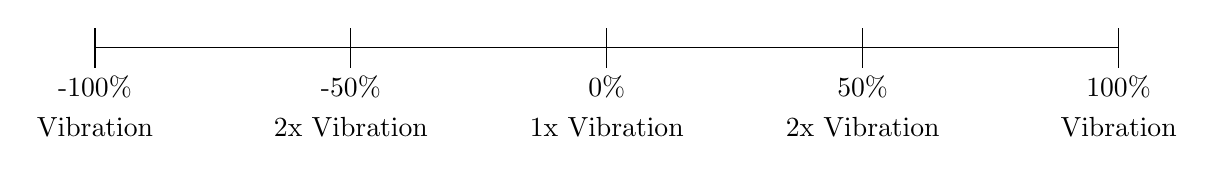
\begin{tikzpicture}
        \draw (0,0) -- (13,0);
        \draw (0,0.25) -- (0,-0.25);
        \draw (0,-0.5) node {-100\%};
        \draw (0,-1) node {Vibration};
        \draw (3.25, 0.25) -- (3.25, -0.25);
        \draw (3.25,-0.5) node {-50\%};
        \draw (3.25,-1) node {2x Vibration};
        \draw (6.5,0.25) -- (6.5,-0.25);
        \draw (6.5,-0.5) node {0\%};
        \draw (6.5,-1) node {1x Vibration};
        \draw (9.75,0.25) -- (9.75,-0.25);
        \draw (9.75,-0.5) node {50\%};
        \draw (9.75,-1) node {2x Vibration};
        \draw (13,0.25) -- (13,-0.25);
        \draw (13,-0.5) node {100\%};
        \draw (13,-1) node {Vibration};
    \end{tikzpicture}
\end{figure}

Dabei ist die Schwelle so gewählt, dass die Vibrationen nicht zu oft ausgelöst werden. 
Es ist wichtig zu wissen, dass der Wert basierend auf der Eingabe des Joysticks kontinuierlich berechnet wird.
Die Eingabe beträgt -1 bis 1. Dabei ist -1 die maximale Position nach links und 1 die maximale Position nach rechts.
Damit die Ruderstellung nicht zu schnell verändert wird, benötigt diese eine volle Eingabe von 1 oder -1 für 2 Sekunden,
damit die Ruderstellung 100\% erreicht. Entsprechend werden die 100\% langsamer erreicht, wenn die Eingabe geringer
ist.

\subsection{CAN-Bus Nachrichtenkodierung} \label{sec:canBus}
Die Kodierung der CAN-Bus Nachrichten ist der Hauptbestandteil des Programms \texttt{canInterpreter.py}, welches im Rahmen dieser Arbeit
entwickelt wurde. 
Das Teilprogramm \texttt{canInterpreter.py} erhält Eingaben von \texttt{controllerInput.py}. Basierend auf den
Eingaben des Xbox-Controllers wird dann die entsprechende Nachricht erstellt. Um eine Nachricht zu kodieren, wird die Bibliothek \texttt{cantools} benutzt.
Mit dieser Bibliothek können DBC-Dateien gelesen und Nachrichten erstellt werden. Mit einer solchen Datei kann eine
bestimmte Nachricht mit ihren Signalen definiert werden. In Kapitel \ref{sec:canTranslation} wurde bereits auf den
Aufbau einer DBC-Datei eingegangen. \\
Bei der Verarbeitung der Eingabe ist es wichtig, dass diese in den richtigen Wertebereich umgewandelt wird.
Beispielsweise dürfen die Umdrehungen pro Minute (RPM) nicht unter 500 liegen, wenn der Motor in Betrieb ist.
Daher wird die Eingabe auf den Wertebereich von 500 bis 2500 Umdrehungen pro Minute umgewandelt. Dieser Bereich
geht aus einer Analyse der aufgezeichneten Nachrichten hervor.
\\
In der benötigten Nachricht ist eine Prüfsumme von 4 Bit notwendig. Jedoch gibt es zwei Methoden der Prüfsummenberechnung
nach dem SAE J1939 Standard \cite{VectorSAE}. Diese Quelle gibt aber auch die richtige Methode für den benötigten Nachrichtentypen
an. Bei dem Nachrichtentyp handelt es sich um eine TSC1-Nachricht. Diese Nachricht wird für die Steuerung der Motoren
benutzt. Allerdings stimmt die Methode nicht mit den aufgezeichneten Nachrichten überein. In den Nachrichten der Limanda
scheint die Prüfsumme nur auf Basis des Nachrichtenzählers bestimmt zu werden. Daher wurde die Prüfsumme nur auf Basis des Nachrichtenzählers
bestimmt und so den aufgezeichneten Nachrichten angepasst.
Am Ende wird die Prüfsumme der Nachricht hinzugefügt und die
Nachricht wird an den CAN-Bus gesendet. \\
Insgesamt sieht die Kodierung einer TSC1-Nachricht wie folgt aus:
\begin{minted}[linenos, fontsize=\footnotesize, frame=lines]{python3}
    def encodeThrottleMessage(speed, throttle, canFrameID):
    torqueHiRes = throttle * 0.125
    if torqueHiRes > 0.875:
        torqueHiRes = 0.875
    throttle = (throttle * 35) - 110 
    # laut aufgezeichneten Werten ist nur bereich von -110 bis -85 bekannt
    if messageCounter != 4 and messageCounter != 15: 
        checksum = 0
    elif messageCounter == 4:
        checksum = 3
    else:
        checksum = 15
    try:
        throttleInput = gasLeverMessage.encode({ 
            'EngOverrideCtrlMode': 3, #3: Speed / Torque Limit Control Mode
            'EngRequestedSpeedCtrlConditions': 0, 
            # 0: Transient Optimized for driveline disengaged and non-lockup conditions
            'OverrideCtrlModePriority': 0, # 0: Highest Priority
            'EngRequestedSpeed_SpeedLimit': speed,
            'EngRequestedTorque_TorqueLimit': throttle,
            'TSC1TransRate': 4, # Transmission Rate of 100ms
            'TSC1CtrlPurpose': 31, # Temporary PowerTrain Control
            'EngRequestedTorqueHighResolution': torqueHiRes,
            'MessageCounter': messageCounter,
            'MessageChecksum': checksum
        })
        return can.Message(arbitration_id=canFrameID, data=throttleInput, is_extended_id=False)
\end{minted}
Wie in dem Code zu sehen ist, werden die Eingaben des Xbox-Controllers vor der Kodierung in den richtigen Wertebereich umgewandelt.
Das passiert in den Zeilen 2--5. Danach wird auf Grundlage des Nachrichtenzählers die Prüfsumme bestimmt. Die genauen Werte wurden 
den aufgezeichneten Nachrichten entnommen. In den Zeilen 14--25 wird die Nachricht erstellt. Dabei werden den Signalen die entsprechenden
Werte zugewiesen. Mithilfe von \texttt{cantools} wird die Nachricht mit einer bestimmten ID erstellt. Nun liegt die Nachricht als
CAN-Nachricht vor und kann an den CAN-Bus gesendet werden.
\\
Zur Überwachung des CAN-Bus wurde das Programm \texttt{canReader.py} entwickelt. Es kann die wichtigen Nachrichten für diese Arbeit 
auf dem CAN-Bus lesen und in Echtzeit dekodieren. Dabei handelt es sich um die Nachrichten für die Motorsteuerung und die Gangschaltung.
Dazu wurde wieder die Bibliothek \texttt{cantools} benutzt. Auch hier wird
mit der gleichen DBC-Datei gearbeitet, da es sich um die gleichen Nachrichten handelt. In den dekodierten Nachrichten
können die Signale und deren Werte gesehen werden. 
In den aufgezeichneten Nachrichten wurde entdeckt, dass Nachrichten für die Motorsteuerung
immer eine PGN von 0 haben. Da nur diese Nachrichten
mit der PGN 0 gesendet werden, kann nach dieser gefiltert werden. Die gefundenen Nachrichten werden dann dekodiert und
spezifisch nach
dem Signal \texttt{'EngRequestedTorque\_TorqueLimit'} durchsucht. 
Das Dekodieren wird mit Hilfe von \texttt{cantools} realisiert. Zuerst wird die ID der Nachricht einem Nachrichtentyp in der DBC-Datei
zugeordnet. Danach wird die Nachricht dekodiert und die Signale und deren Werte ausgegeben.
Wenn das gesuchte Signal entdeckt wird, dann muss eine eigene Nachricht
gesendet werden, um die wahren Eingaben zu verhindern
Dies passiert wieder durch \texttt{canInterpreter.py} nach 
einem über Pipes übermittelten Signal. Um hier zu verhindern, dass eigene Nachrichten vom eigenen System erkannt werden,
wird ein eigener Identifier benutzt. Das allgemeine Problem wurde bereits in Kapitel \ref{sec:manipulationGashebel}
betrachtet.
Um den Identifier zu berechnen, wurde mit einer Portierung von \texttt{canboatjs} auf Python gearbeitet 
\cite{canboatjs}. 
In diesem Programm kann eine bestehende CAN-ID in Quelle, Priorität und PGN aufgeteilt werden. Diese Werte können dann
einzeln verändert werden. Mit diesen Werten kann dann eine neue CAN-ID berechnet werden. 
Damit werden im eigenen Code die Quelladresse verändert, während die PGN beibehalten wird.
Nun können eigene Nachrichten 
anhand der CAN-ID erkannt werden.\\
Für die Gangschaltung musste eigene Nachricht in der DBC-Datei definiert werden. Hierfür konnte auf die Bedienungsanleitung
des Motors zurückgegriffen werden. In dieser sind die Nachrichten für die Gangschaltung definiert.
Die Nachrichten wurden dann in \texttt{canInterpreter.py} erstellt und gesendet.
Dabei hat sich eine Schwierigkeit ergeben, als die ID nicht als erweiterter J1939-Standard von \texttt{cantools} erkannt wurde. 
Dafür wurde eine Lösung gefunden, indem die ID mit der Hexadezimalen Zahl 80000000 addiert wurde. Mit der Addition dieser Zahl
wird in der binären Darstellung das erste Bit von 0 auf 1 gesetzt. Alternativ kann bei der binären Darstellung der ID das erste Bit
manuell auf 1 gesetzt werden. Die neu erzeugte ID
wird nun ohne Probleme als erweiterte ID erkannt. Diese Lösung konnte nicht in einer offiziellen Dokumentation für den
DBC-Standard gefunden werden. In einem Forum wurde berichtet, dass diese Lösung funktioniert \cite{cantoolsIssue}. 
Zusätzlich hat diese Lösung im Anwendungsfall dieser Arbeit funktioniert. 
Laut der gleichen Quelle hängt der Grund dafür damit zusammen, dass ein Bit für die ID in dem Dateiformat zweckentfremdet für
die Erkennung einer erweiterten ID benutzt wird. Allerdings kann dies nicht bestätigt werden. \\
Da in der Nachricht für das Getriebe auch die aktuelle maximale zulässige Last (\texttt{'CurrentMaxPermissibleLoad'}) gesendet wird, 
reicht es nicht aus, diese
Nachricht nur bei einer Änderung des Gangs zu senden. Daher wird die Nachricht bei jeder Änderung der Gashebelposition
gesendet. Damit hat die aktuelle maximale zulässige Last immer den aktuellen Wert der Eingabe des Xbox-Controllers.